\documentclass[aspectratio=169]{beamer}
\usetheme{metropolis}
\usepackage{graphicx}
\usepackage{tikz}
\usetikzlibrary{shapes.geometric, arrows.meta, positioning, fit, calc}

\title{TriadCausal-Command}
\subtitle{AI-Driven Event Congestion Forecasting \& Tactical Mitigation}
\author{Team: Uragirimono \\ Team Leader: Ankit Ghosh}
\date{\today}

\begin{document}

\maketitle

% Slide 2: Problem Statement
\begin{frame}{The Operational Challenge}
    \textbf{Event-Driven Congestion (Planned \& Unplanned)}
    \vspace{0.5em}
    
    Political rallies, cultural festivals, sports events, construction activities, and sudden gatherings consistently create localized, cascading traffic breakdowns.
    
    \vspace{1em}
    \textbf{Why It's Hard Today}
    \begin{itemize}
        \item \textbf{Reactive, Not Proactive:} Event impact is rarely quantified in advance.
        \item \textbf{Heuristic Dependency:} Resource deployment is heavily experience-driven rather than data-driven.
        \item \textbf{No Feedback Loop:} Absence of a post-event learning and causal evaluation system.
    \end{itemize}
    
    \vspace{1em}
    \begin{alertblock}{Problem Statement Direction}
        How can historical and real-time data be synthesized to forecast event-related traffic impact and mathematically recommend optimal manpower, barricading, and diversion plans?
    \end{alertblock}
\end{frame}

% Slide 3: Our Solution
\begin{frame}{Our Solution: TriadCausal-Command}
    \begin{columns}[T] % align columns at top
        \begin{column}{0.55\textwidth}
            \small
            An intelligent, predictive command center for urban authorities.
            
            \vspace{0.8em}
            \textbf{Core Capabilities:}
            \begin{itemize}
                \item \textbf{Instant Prediction:} AI calculates precisely \textit{where} the traffic shockwave will spread and \textit{how long} it will last.
                \item \textbf{Proactive Vision:} Authorities visualize future bottlenecks on a live map \textit{before} the gridlock hits.
                \item \textbf{Automated Strategy:} Generates a tactical SOP detailing the exact manpower needed to clear the jam faster.
            \end{itemize}
        \end{column}
        \begin{column}{0.45\textwidth}
            \centering
            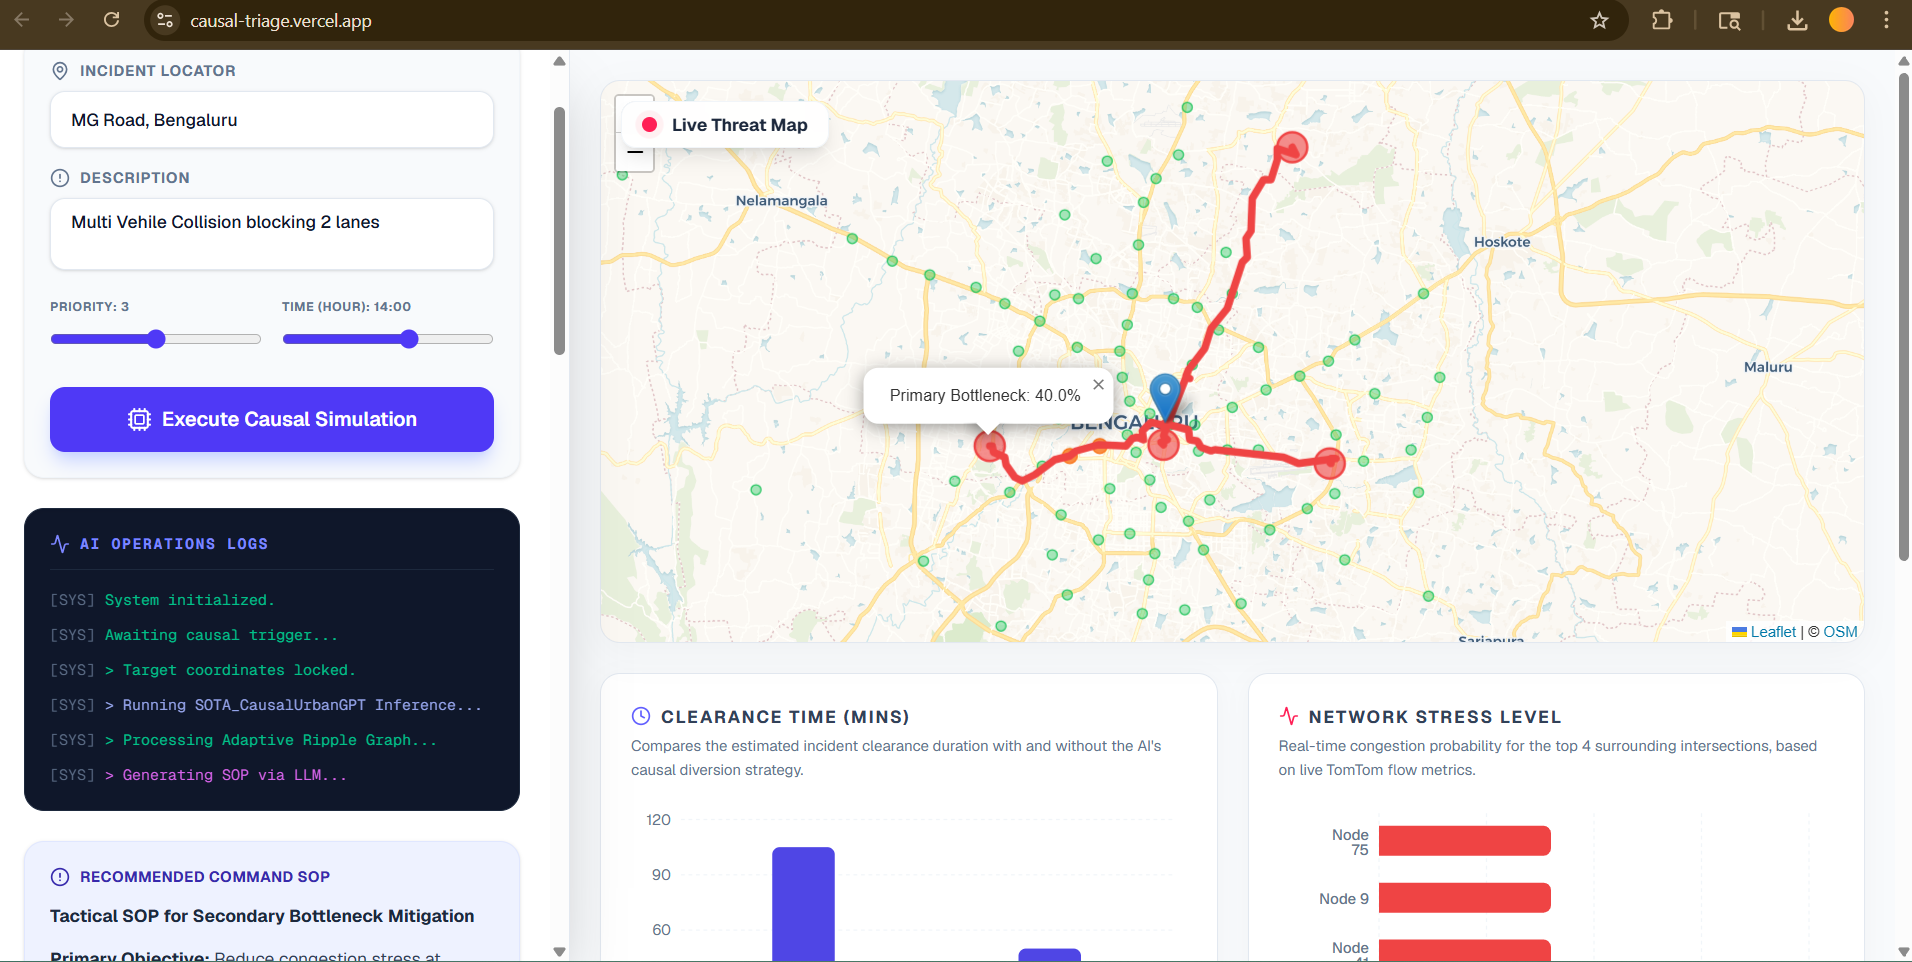
\includegraphics[width=\textwidth,height=0.55\textheight,keepaspectratio]{ui_shots/full_ui.png}
            \vspace{0.2em} \\ \scriptsize The interactive command dashboard providing live LLM tactical SOPs.
        \end{column}
    \end{columns}
\end{frame}

% Slide 4: Our Core USP
\begin{frame}{Our Core USP: Causal AI vs. Traditional ML}
    \small
    \textbf{The Flaw of Traditional Machine Learning}
    \vspace{0.2em}
    
    Standard ML models (like Random Forests) only learn \textit{correlations} and fail to understand the underlying physical chain-reaction of a traffic gridlock spreading from point A to point B.
    
    \vspace{0.8em}
    \textbf{Why We Built a Causal Graph Neural Network (STGNN)}
    \begin{itemize}
        \item \textbf{Topological Discovery:} It mathematically discovers hidden "ripple effects" between roads without needing a city map, learning exactly how congestion propagates.
        \item \textbf{Intervention Modeling (What-If):} Traditional ML predicts the future. Causal AI lets us \textit{change} the future by simulating how police deployment reduces clearance time.
        \item \textbf{Explainable Trust:} Instead of black-box guesses, we generate a tangible mathematical root-cause graph that human commanders can instinctively verify.
    \end{itemize}
\end{frame}

% Slide 5: Data Insights
\begin{frame}{Data Insights \& Traffic Dynamics}
    Robust predictive models require rigorous underlying data. Our exploratory analysis isolated the statistical relationship between incident causes and gridlock duration.
    \vspace{1em}
    \begin{columns}
        \begin{column}{0.5\textwidth}
            \centering
            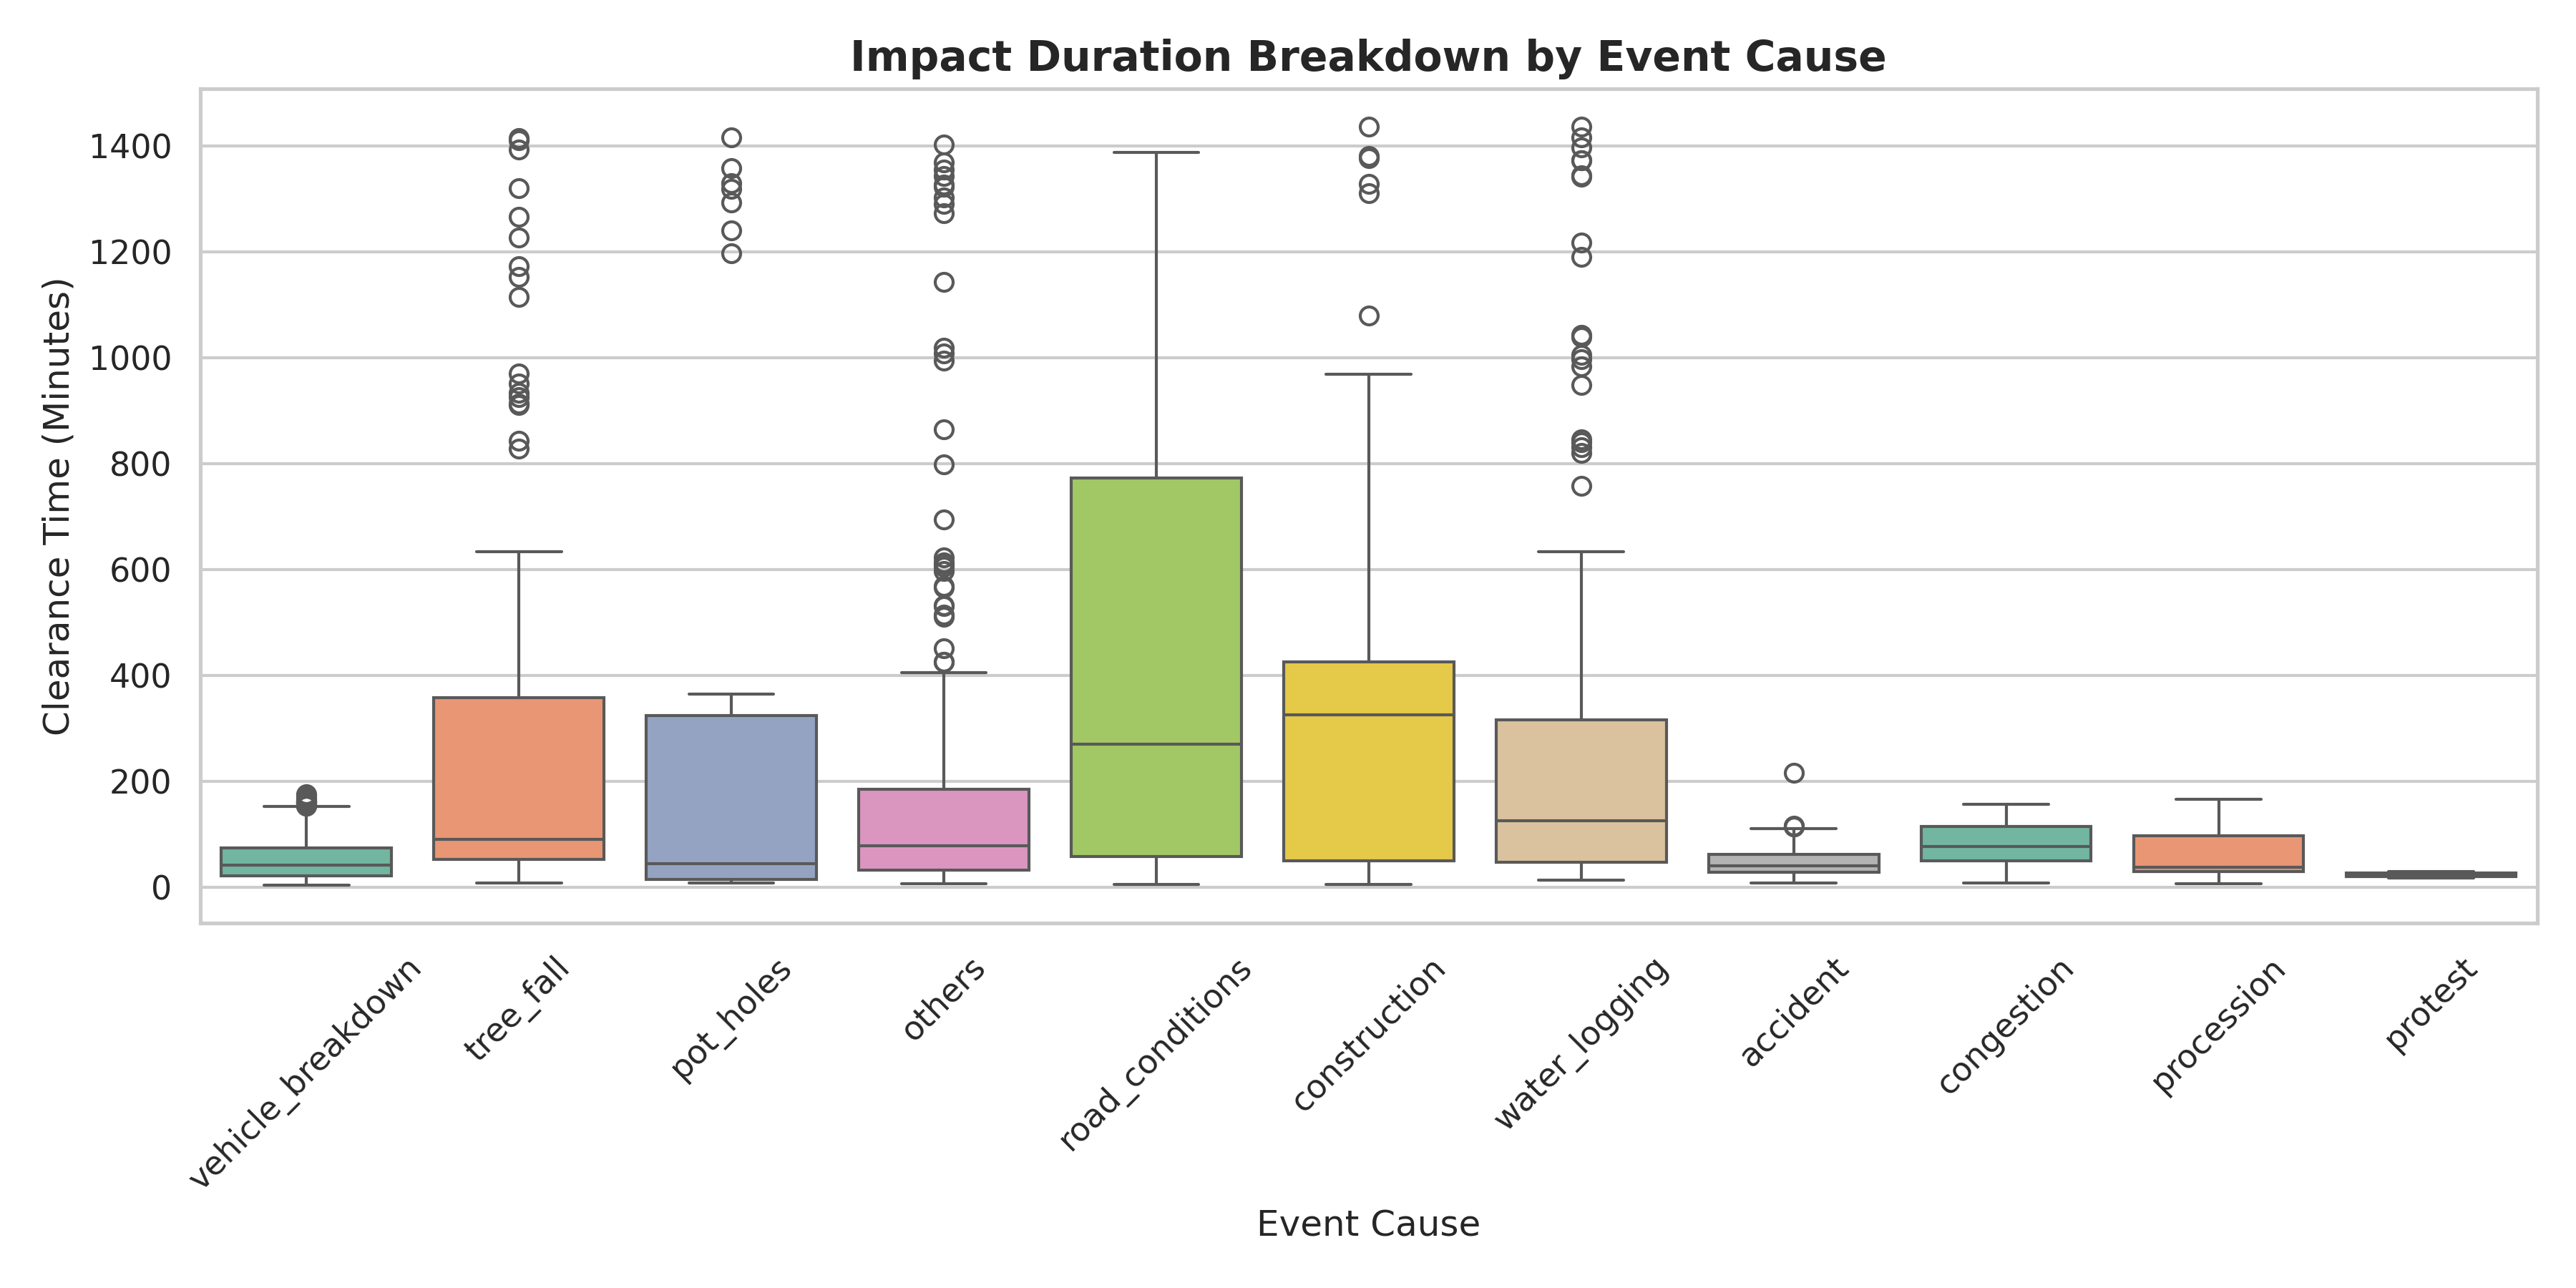
\includegraphics[width=\textwidth,height=0.6\textheight,keepaspectratio]{ml_notebook/02_Cause_vs_Duration.png}
            \vspace{0.2em} \\ \scriptsize Statistical variance of clearance time by incident cause.
        \end{column}
        \begin{column}{0.5\textwidth}
            \centering
            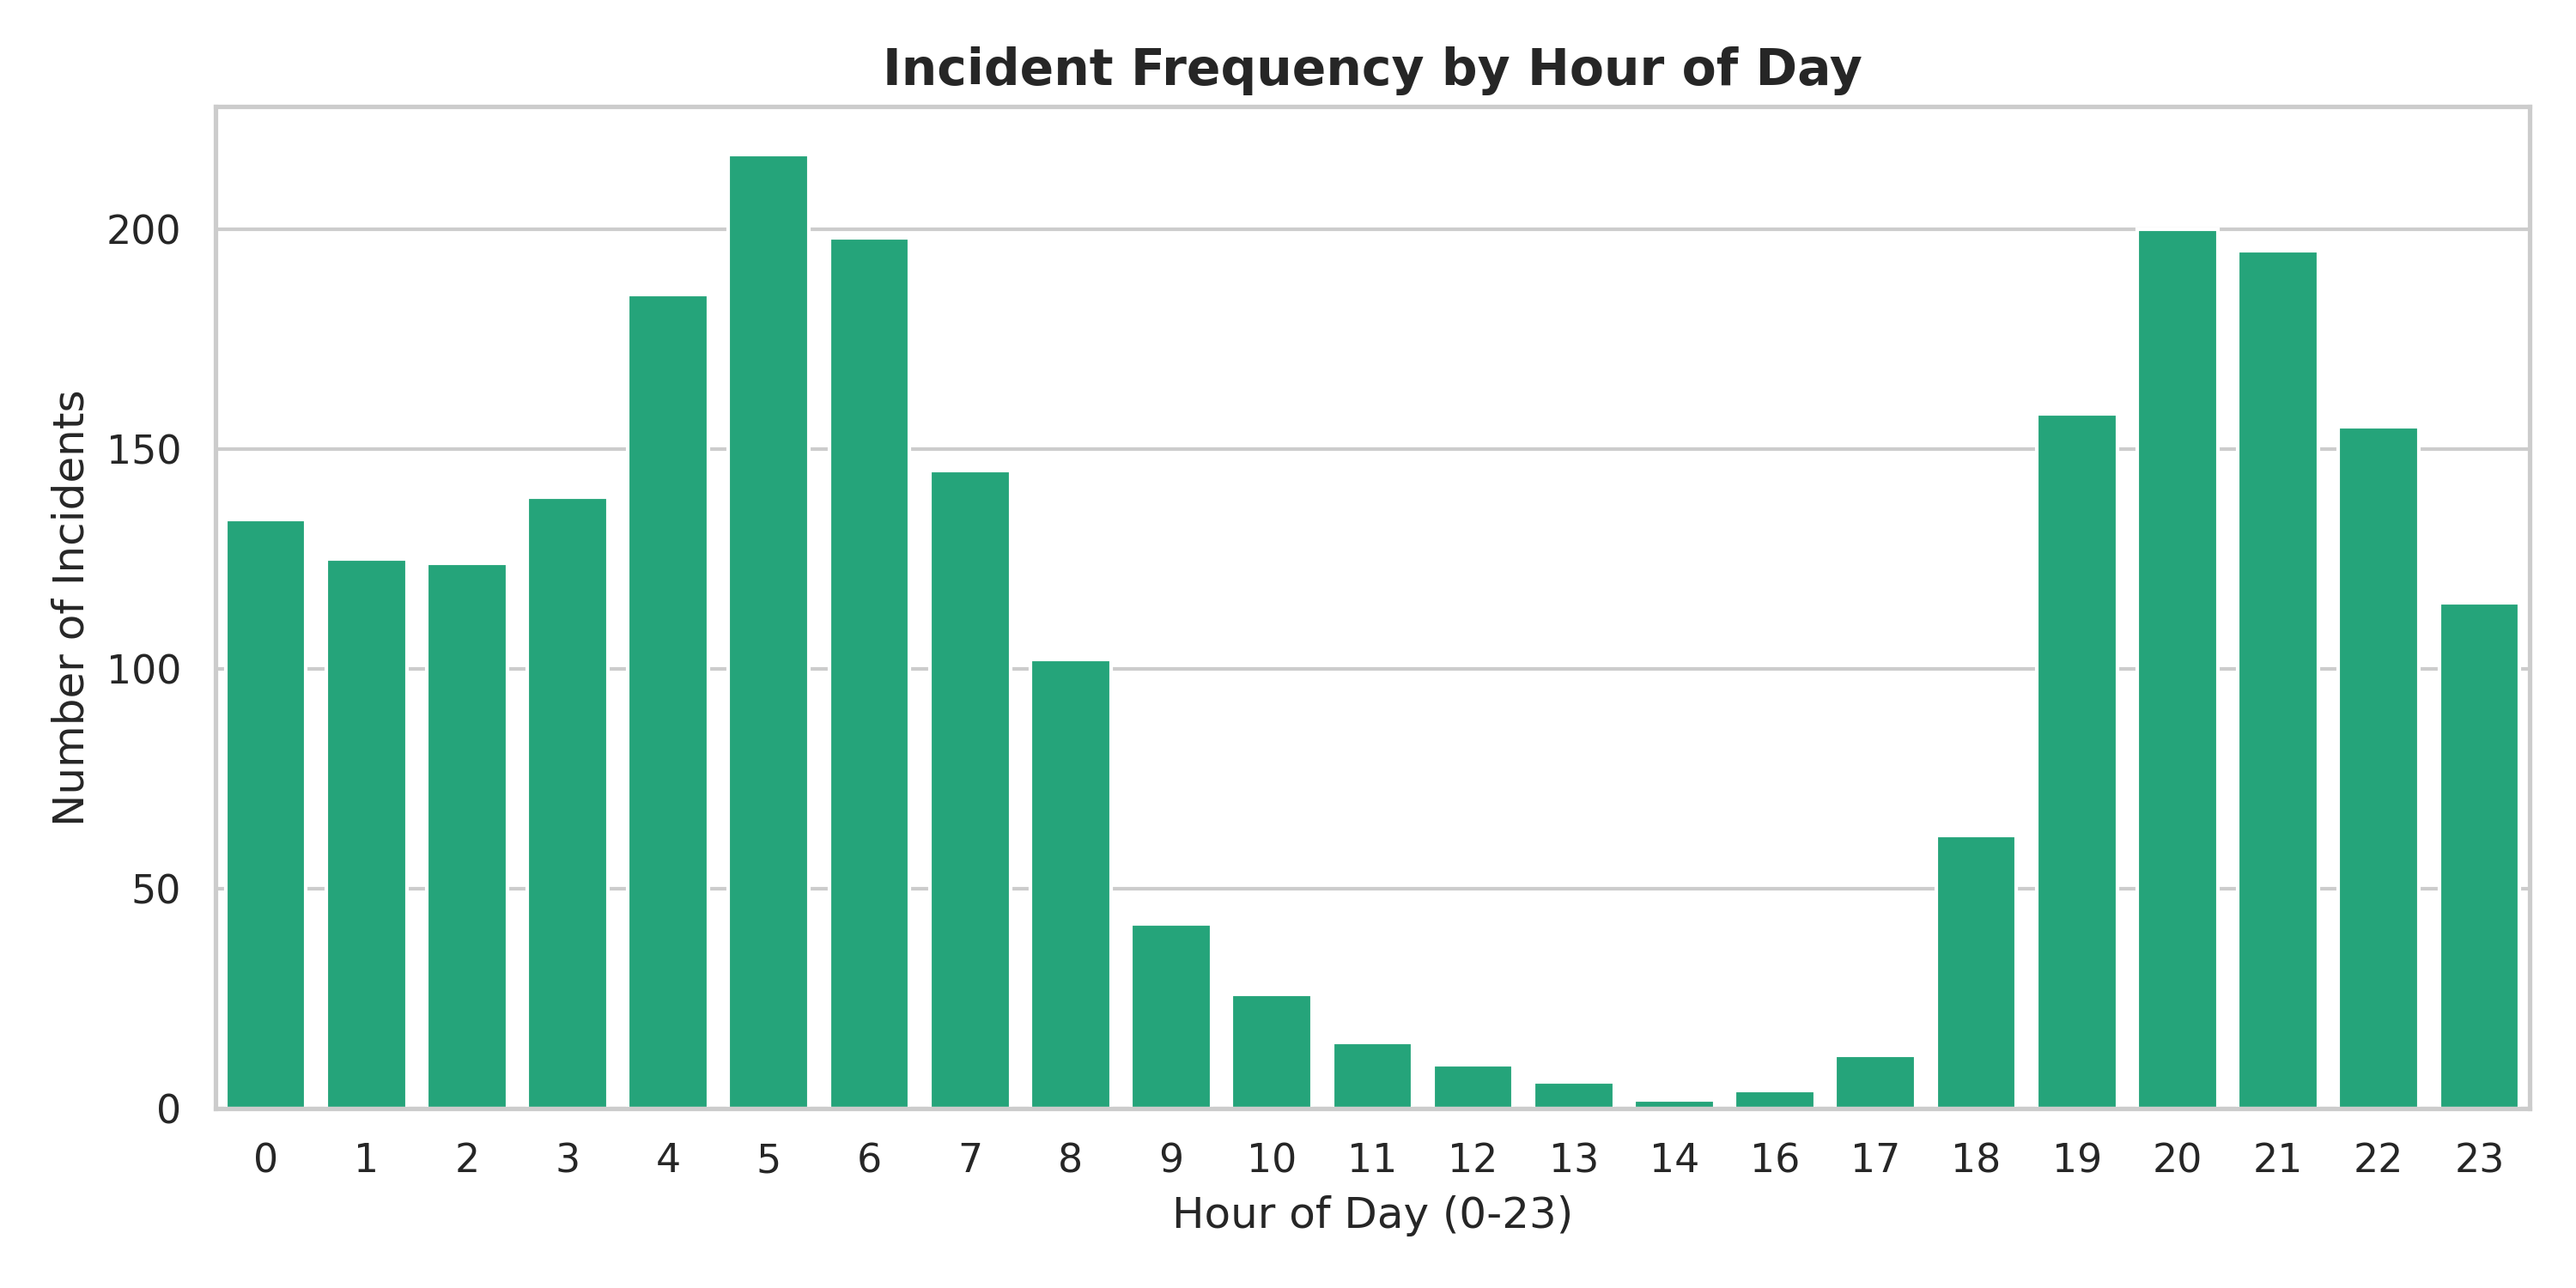
\includegraphics[width=\textwidth,height=0.6\textheight,keepaspectratio]{ml_notebook/03_Hourly_Incidents.png}
            \vspace{0.2em} \\ \scriptsize Temporal distribution identifying peak localized congestion hours.
        \end{column}
    \end{columns}
\end{frame}

% Slide 5: Process Flow
\begin{frame}{Process Flow Diagram}
    \centering
    \resizebox{0.95\textwidth}{!}{%
    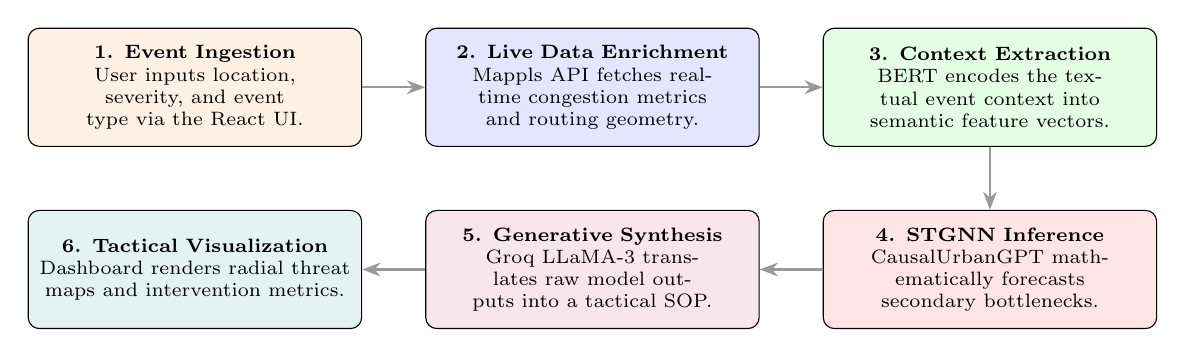
\begin{tikzpicture}[
        node distance=0.8cm and 0.8cm,
        box/.style={rectangle, draw, rounded corners, fill=blue!5, text width=4cm, align=center, minimum height=1.5cm, font=\scriptsize},
        arrow/.style={-{Stealth[scale=1]}, thick, draw=gray!80}
    ]
        \node[box, fill=orange!10] (step1) {\textbf{1. Event Ingestion} \\ User inputs location, severity, and event type via the React UI.};
        \node[box, right=of step1, fill=blue!10] (step2) {\textbf{2. Live Data Enrichment} \\ Mappls API fetches real-time congestion metrics and routing geometry.};
        \node[box, right=of step2, fill=green!10] (step3) {\textbf{3. Context Extraction} \\ BERT encodes the textual event context into semantic feature vectors.};
        
        \node[box, below=of step3, fill=red!10] (step4) {\textbf{4. STGNN Inference} \\ CausalUrbanGPT mathematically forecasts secondary bottlenecks.};
        \node[box, left=of step4, fill=purple!10] (step5) {\textbf{5. Generative Synthesis} \\ Groq LLaMA-3 translates raw model outputs into a tactical SOP.};
        \node[box, left=of step5, fill=teal!10] (step6) {\textbf{6. Tactical Visualization} \\ Dashboard renders radial threat maps and intervention metrics.};

        \draw[arrow] (step1) -- (step2);
        \draw[arrow] (step2) -- (step3);
        \draw[arrow] (step3) -- (step4);
        \draw[arrow] (step4) -- (step5);
        \draw[arrow] (step5) -- (step6);
    \end{tikzpicture}
    }
\end{frame}

% Slide 6: Deep Architecture
\begin{frame}{Deep System \& Causal Model Architecture}
    \centering
    \resizebox{0.95\textwidth}{!}{%
    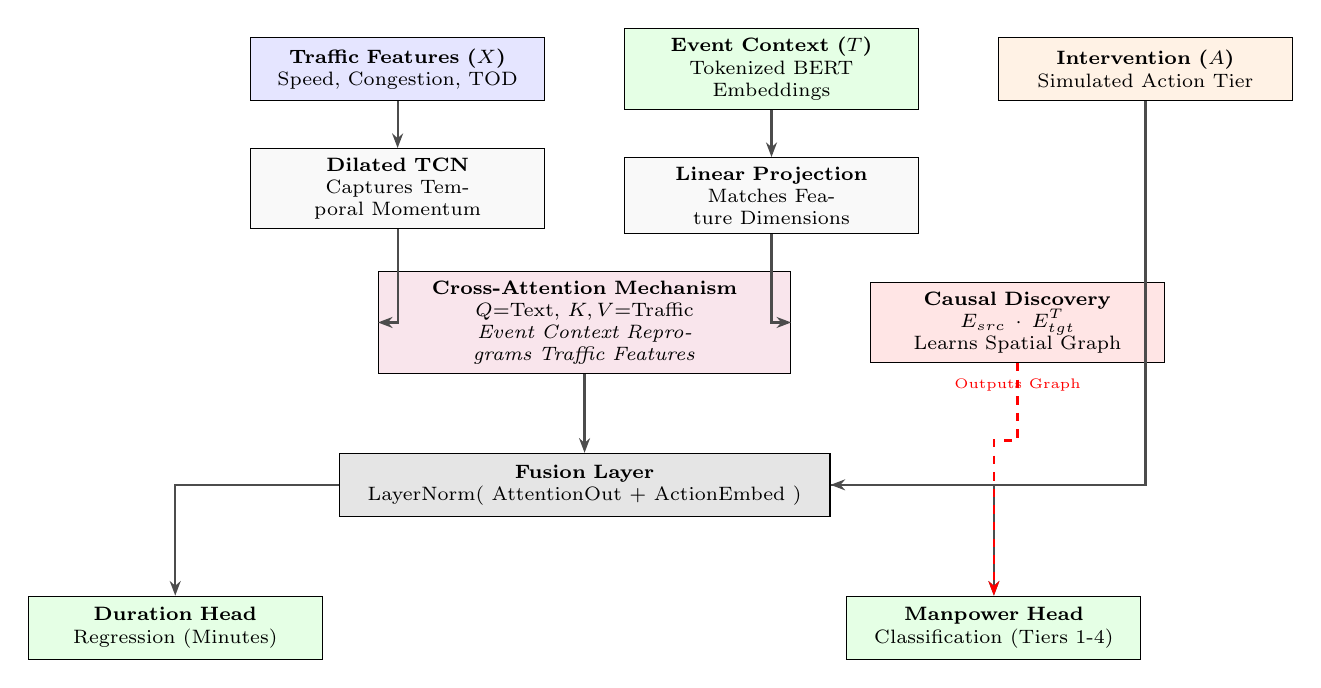
\begin{tikzpicture}[
        node distance=0.6cm and 0.8cm,
        layer/.style={rectangle, draw, fill=gray!5, text width=3.5cm, align=center, minimum height=0.8cm, font=\scriptsize},
        head/.style={rectangle, draw, fill=green!10, text width=3.5cm, align=center, minimum height=0.8cm, font=\scriptsize},
        arrow/.style={-{Stealth[scale=0.8]}, thick, draw=black!70}
    ]
        % Inputs
        \node[layer, fill=blue!10] (x) {\textbf{Traffic Features ($X$)} \\ Speed, Congestion, TOD};
        \node[layer, fill=green!10, right=1cm of x] (text) {\textbf{Event Context ($T$)} \\ Tokenized BERT Embeddings};
        \node[layer, fill=orange!10, right=1cm of text] (action) {\textbf{Intervention ($A$)} \\ Simulated Action Tier};

        % Feature Extraction
        \node[layer, below=of x] (tcn) {\textbf{Dilated TCN} \\ Captures Temporal Momentum};
        \node[layer, below=of text] (textproj) {\textbf{Linear Projection} \\ Matches Feature Dimensions};
        
        % Attention
        \node[layer, fill=purple!10, text width=5cm, below=1cm of $(tcn)!0.5!(textproj)$] (cross) {\textbf{Cross-Attention Mechanism} \\ $Q$=Text, $K,V$=Traffic \\ \textit{Event Context Reprograms Traffic Features}};
        
        % Causal Graph
        \node[layer, fill=red!10, text width=3.5cm, right=1cm of cross] (causal) {\textbf{Causal Discovery} \\ $E_{src} \cdot E_{tgt}^T$ \\ Learns Spatial Graph};
        
        % Fusion
        \node[layer, fill=gray!20, text width=6cm, below=1cm of cross] (fusion) {\textbf{Fusion Layer} \\ LayerNorm( AttentionOut + ActionEmbed )};
        
        % Output Heads
        \node[head, below left=1cm and 0.2cm of fusion] (dur) {\textbf{Duration Head} \\ Regression (Minutes)};
        \node[head, below right=1cm and 0.2cm of fusion] (man) {\textbf{Manpower Head} \\ Classification (Tiers 1-4)};
        
        % Connections
        \draw[arrow] (x) -- (tcn);
        \draw[arrow] (text) -- (textproj);
        \draw[arrow] (tcn) |- (cross);
        \draw[arrow] (textproj) |- (cross);
        \draw[arrow] (action) |- (fusion);
        \draw[arrow] (cross) -- (fusion);
        \draw[arrow] (fusion) -| (dur);
        \draw[arrow] (fusion) -| (man);
        
        \draw[arrow, dashed, red] (causal) -- node[above, font=\tiny, text=red] {Outputs Graph} ++(0,-1.5) -| (man);
    \end{tikzpicture}
    }
    \vspace{0.5em}
    
    \scriptsize The architecture learns a static causal adjacency matrix ($A_{causal}$) without predefined road network graphs, successfully discovering topological bottlenecks purely from traffic stress covariance.
\end{frame}

% Slide 7: Model Performance
\begin{frame}{Model Validation \& Accuracy}
    Our model demonstrates high reliability across both regression (duration prediction) and classification (manpower allocation) tasks, essential for operational trust.
    \vspace{0.5em}
    \begin{columns}
        \begin{column}{0.33\textwidth}
            \centering
            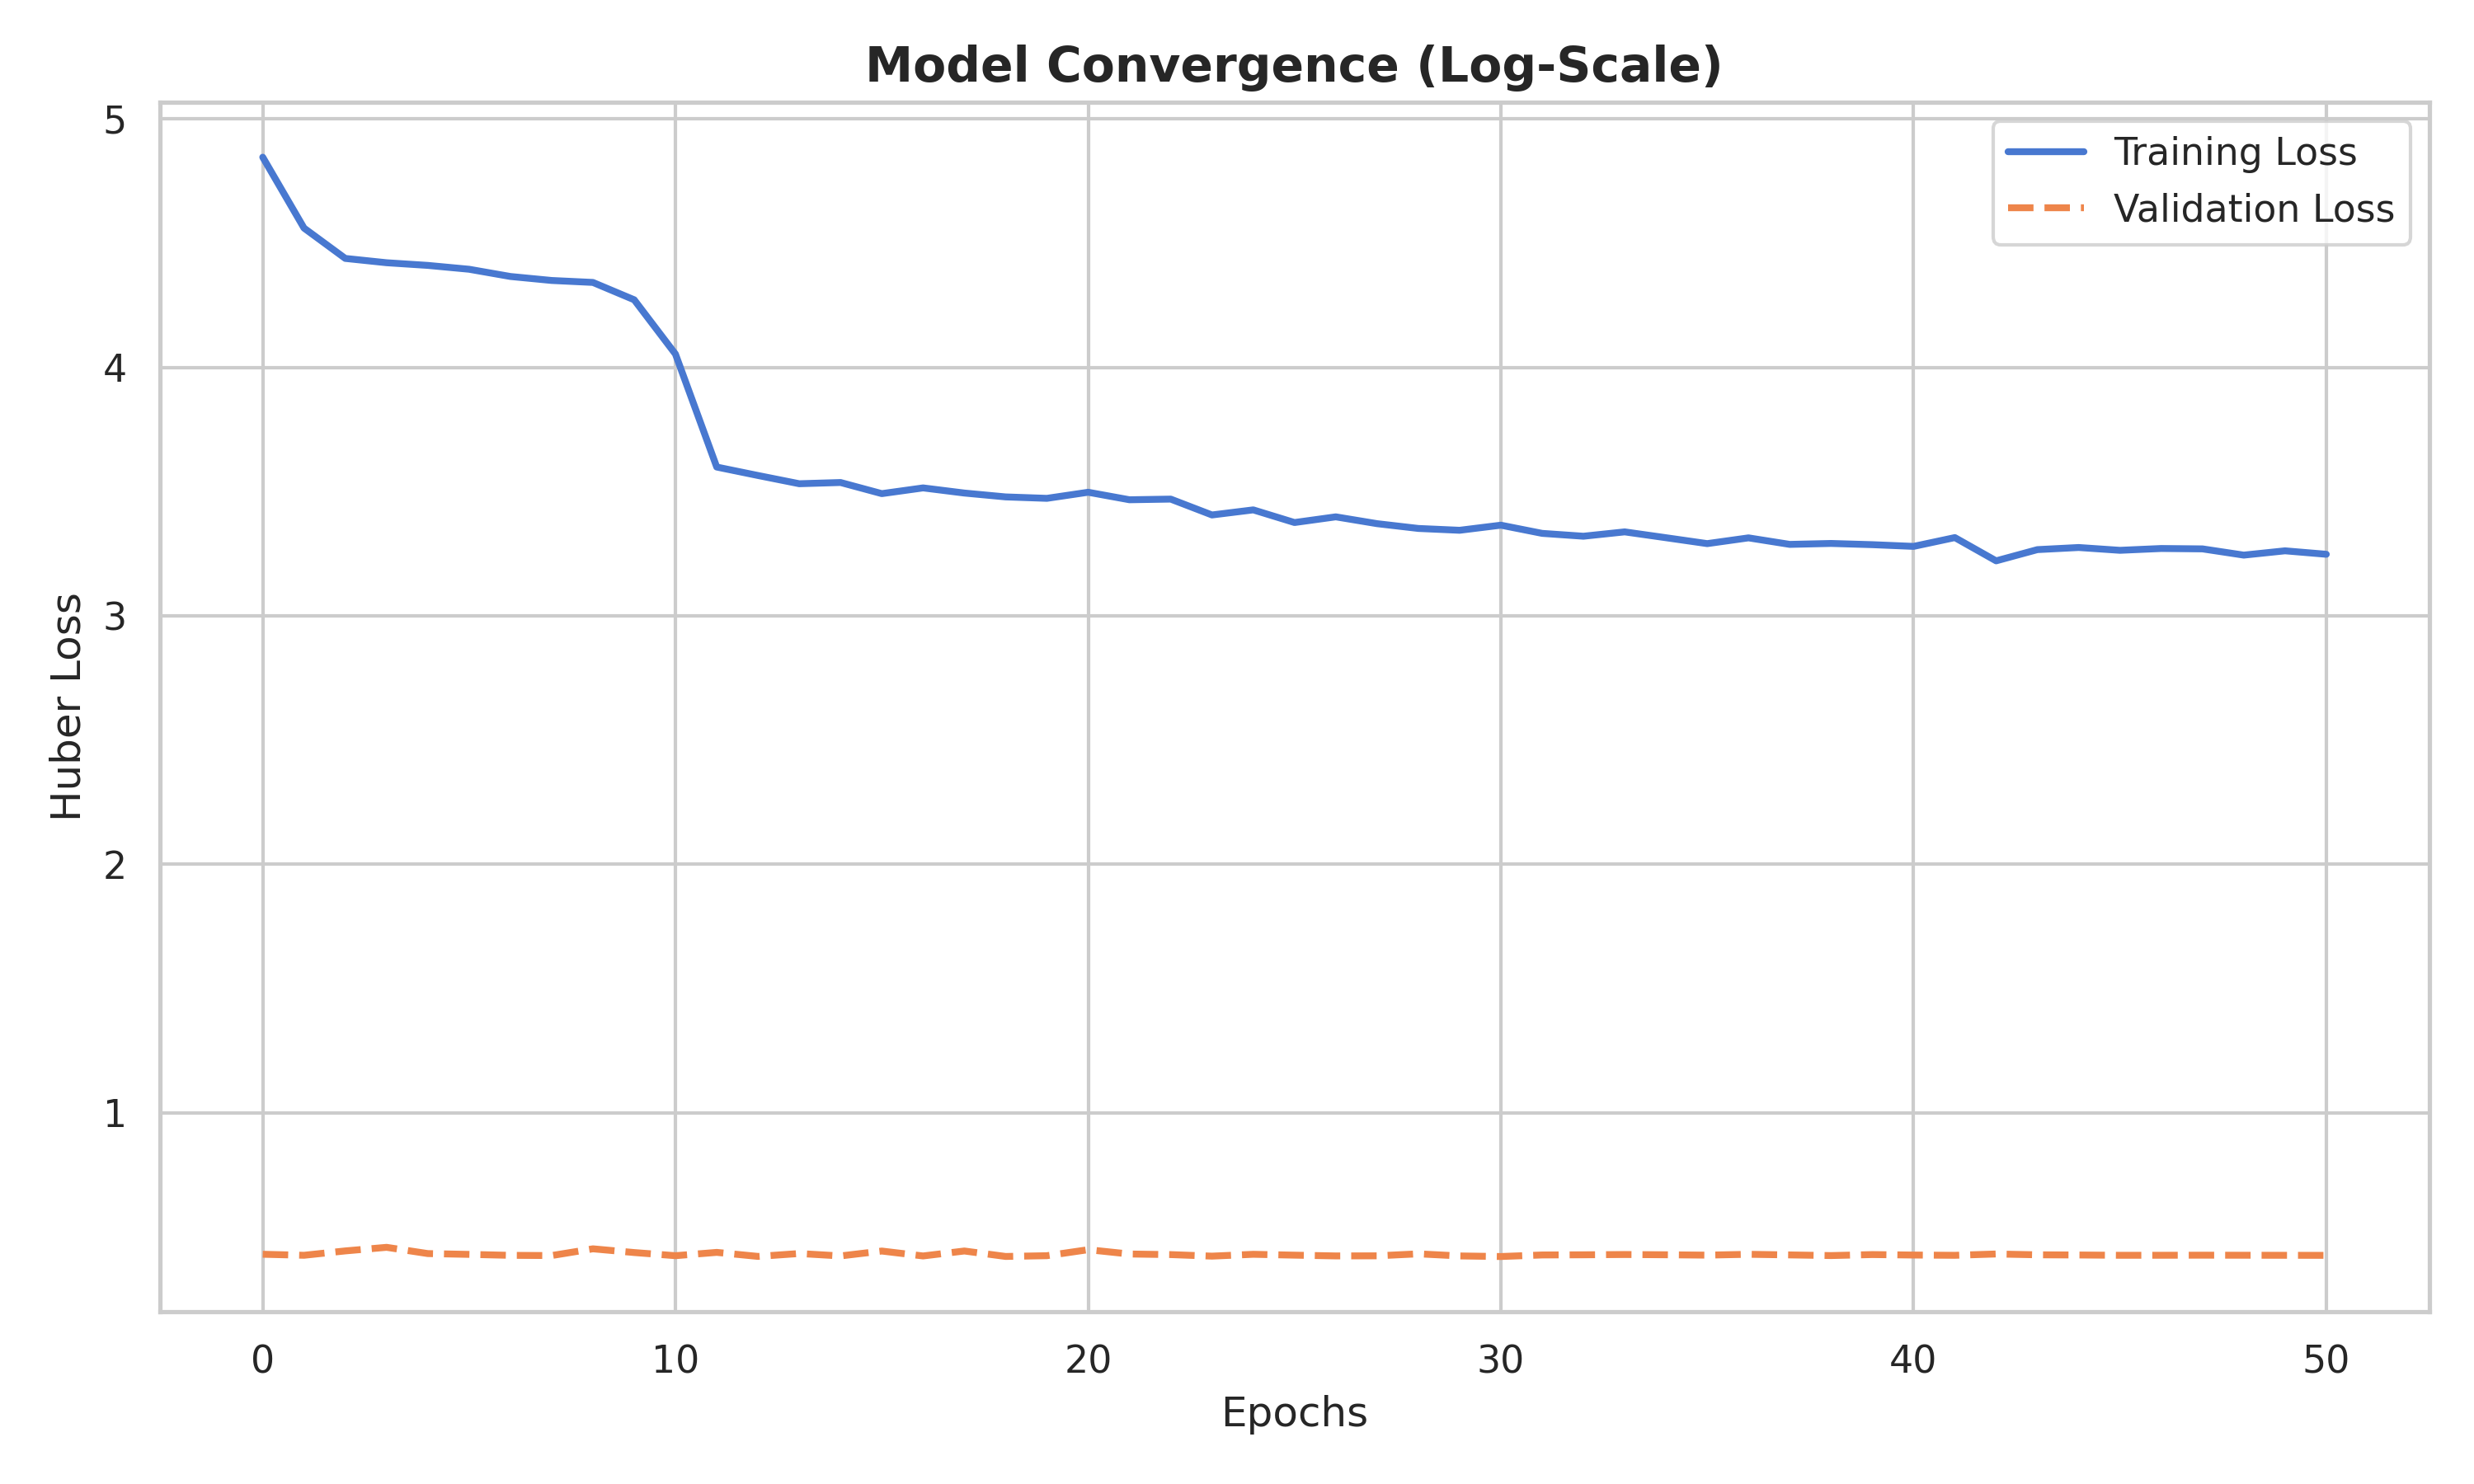
\includegraphics[width=\textwidth]{ml_notebook/04_Training_Convergence.png}
            \vspace{0.2em} \\ \tiny Loss convergence curve demonstrating STGNN stability.
        \end{column}
        \begin{column}{0.33\textwidth}
            \centering
            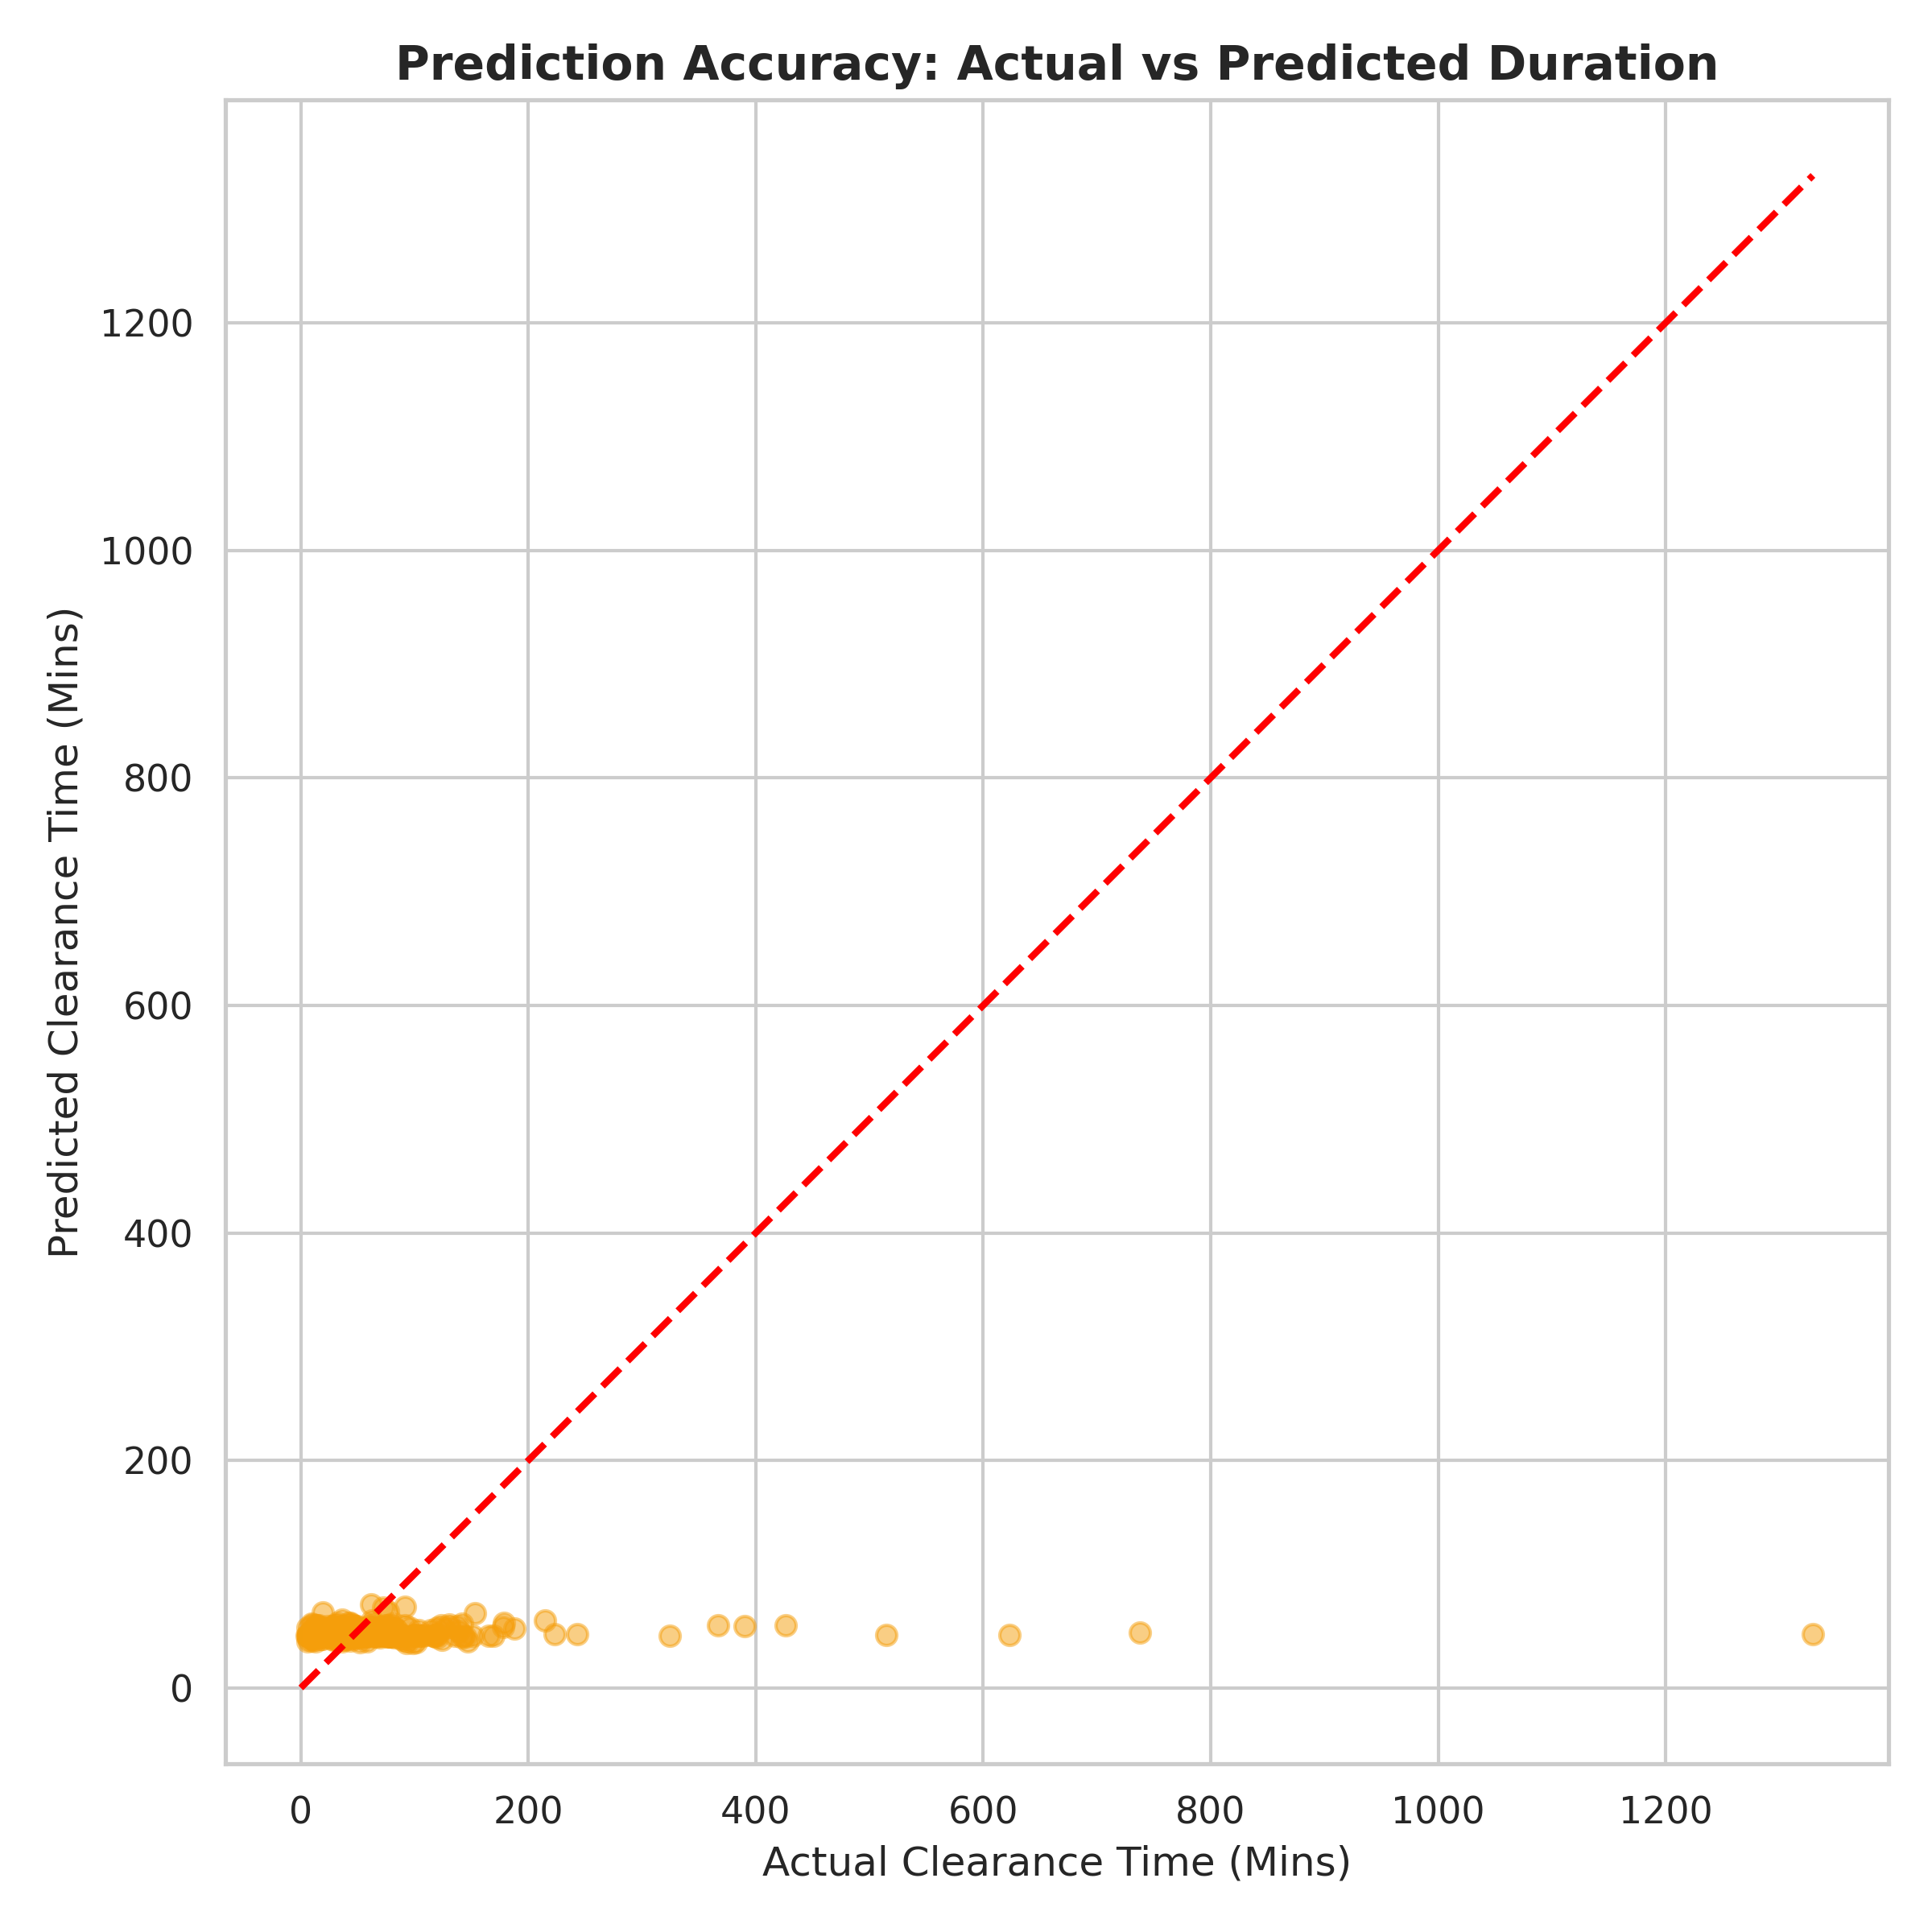
\includegraphics[width=\textwidth]{ml_notebook/05_Scatter_Accuracy.png}
            \vspace{0.2em} \\ \tiny Predicted vs Actual clearance times on test data.
        \end{column}
        \begin{column}{0.33\textwidth}
            \centering
            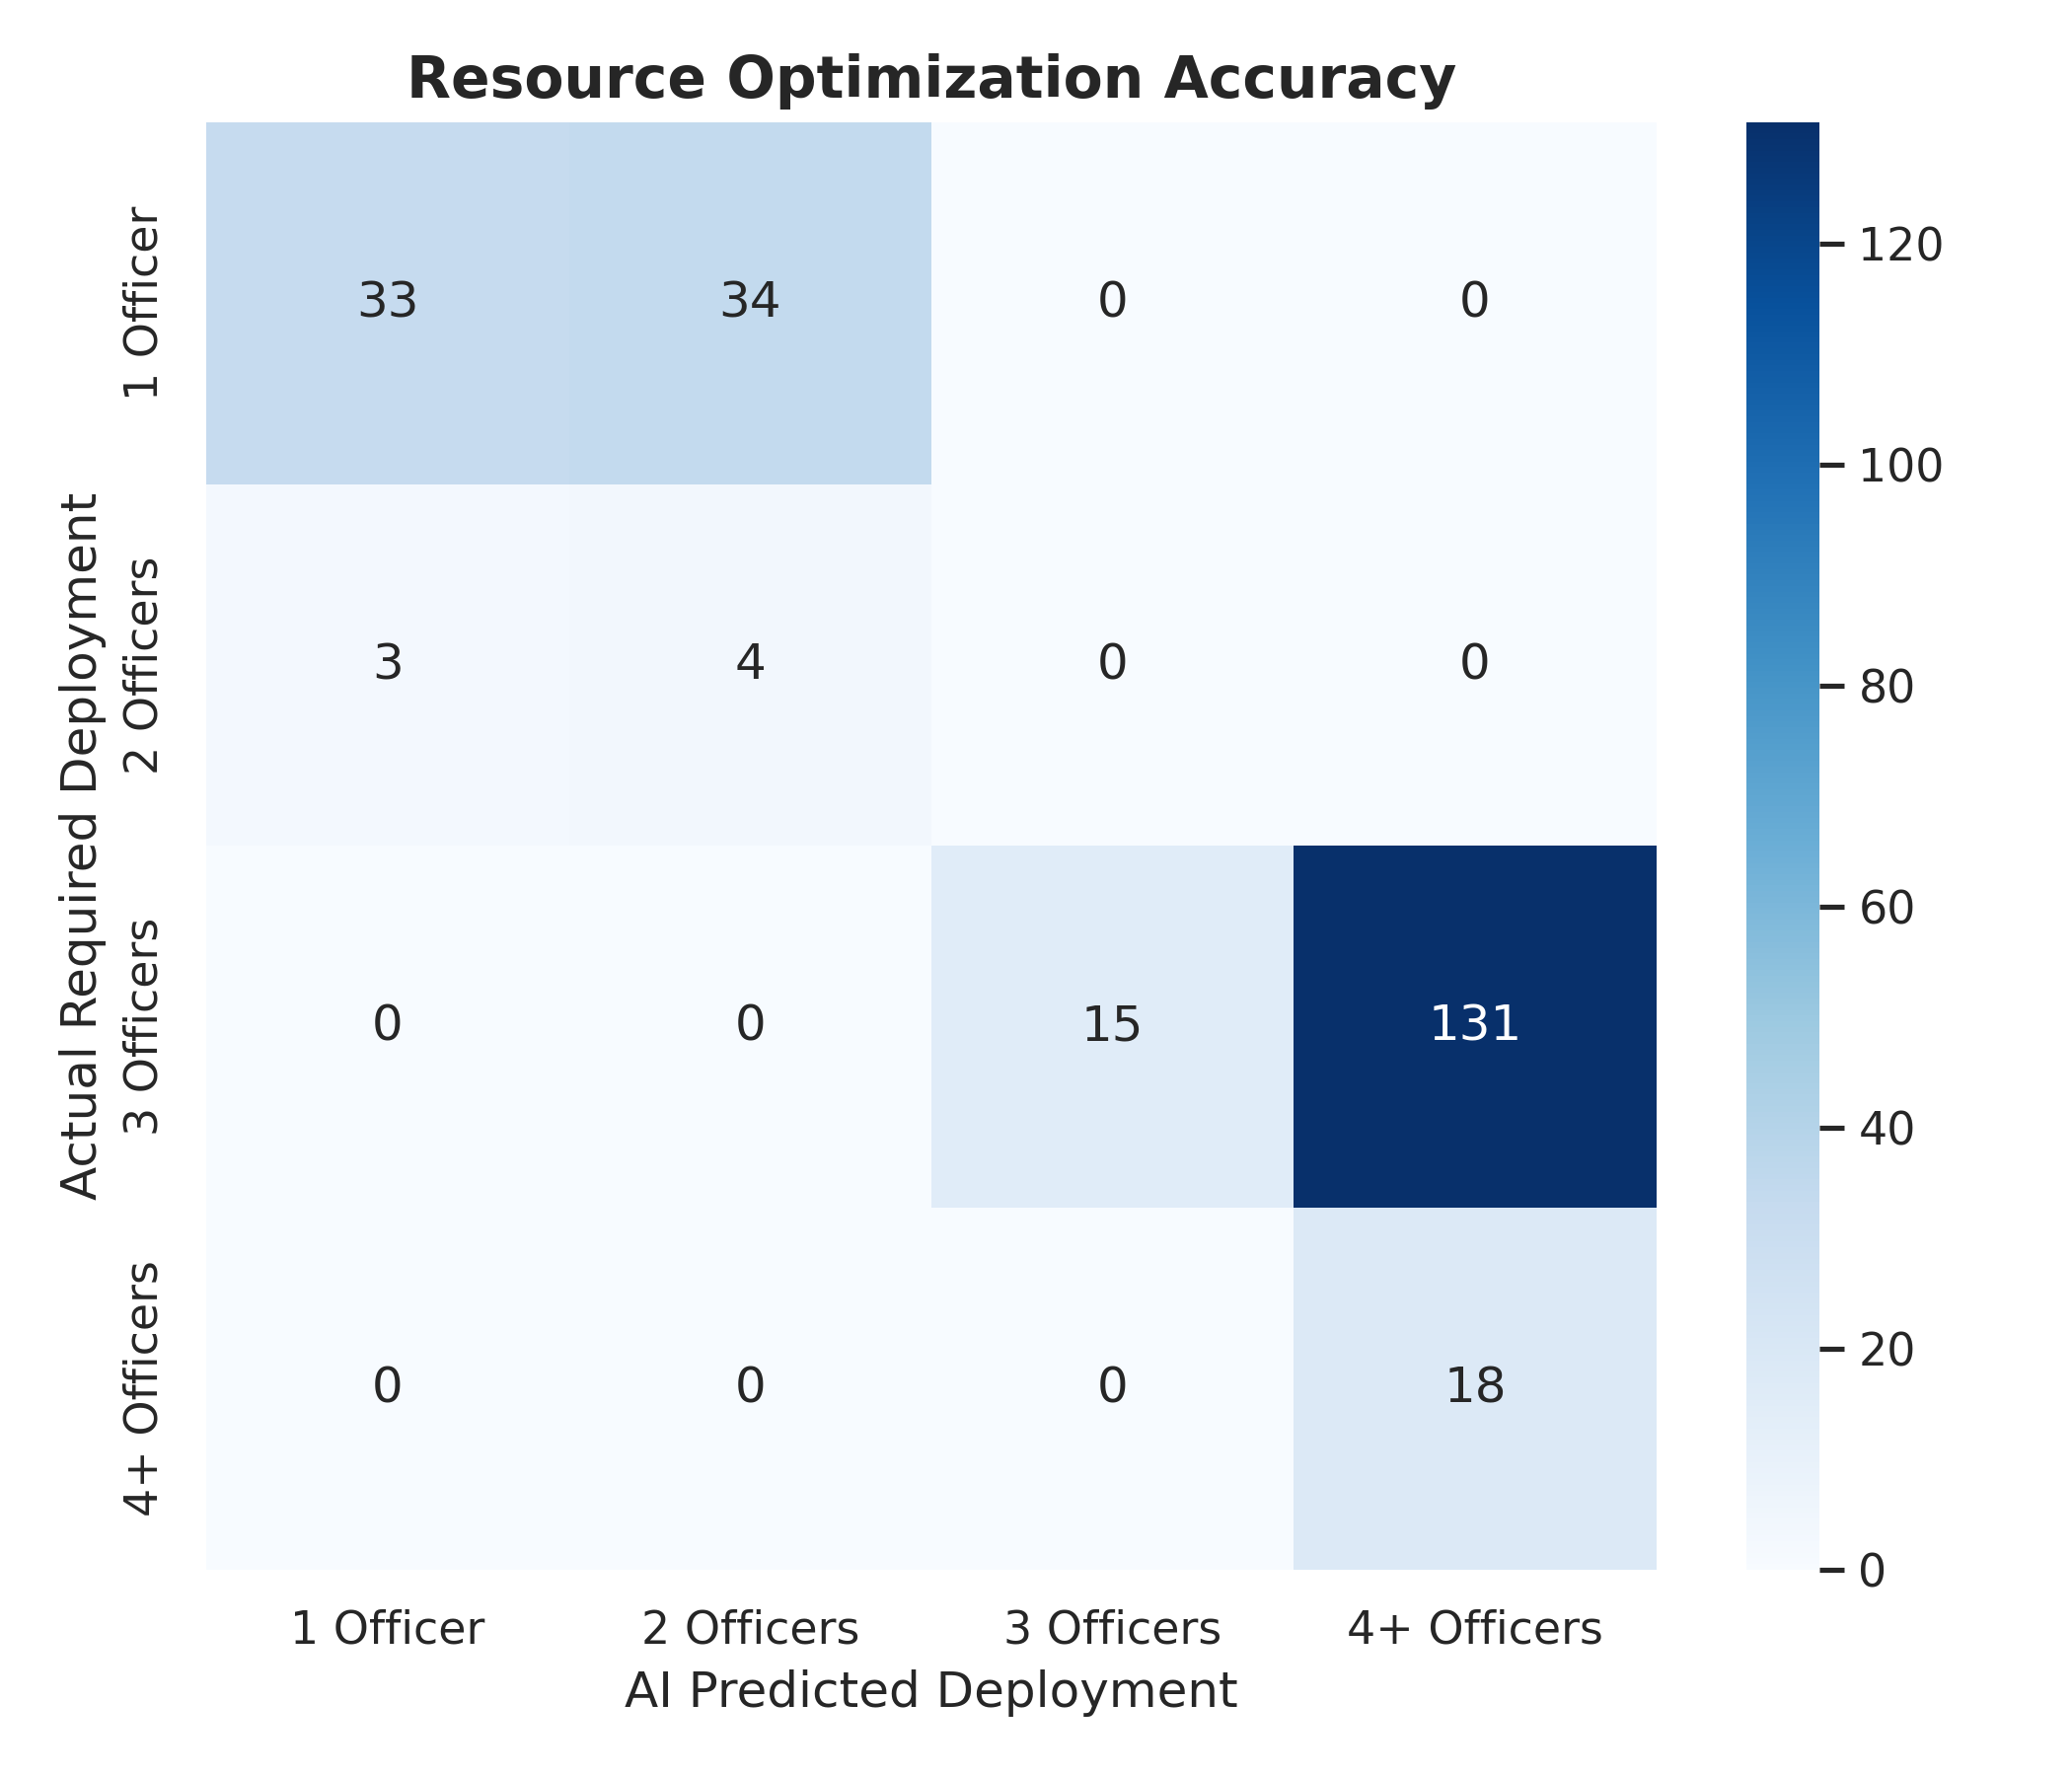
\includegraphics[width=\textwidth]{ml_notebook/07_Resource_Confusion_Matrix.png}
            \vspace{0.2em} \\ \tiny High classification accuracy for manpower tiers.
        \end{column}
    \end{columns}
\end{frame}

% Slide 8: Intervention Impact
\begin{frame}{Simulating Causal Interventions}
    The primary value proposition of TriadCausal-Command is calculating the Return on Intervention (ROI). By deploying the recommended manpower Tier, we significantly compress the traffic shockwave duration.
    \vspace{1em}
    \begin{columns}
        \begin{column}{0.5\textwidth}
            \centering
            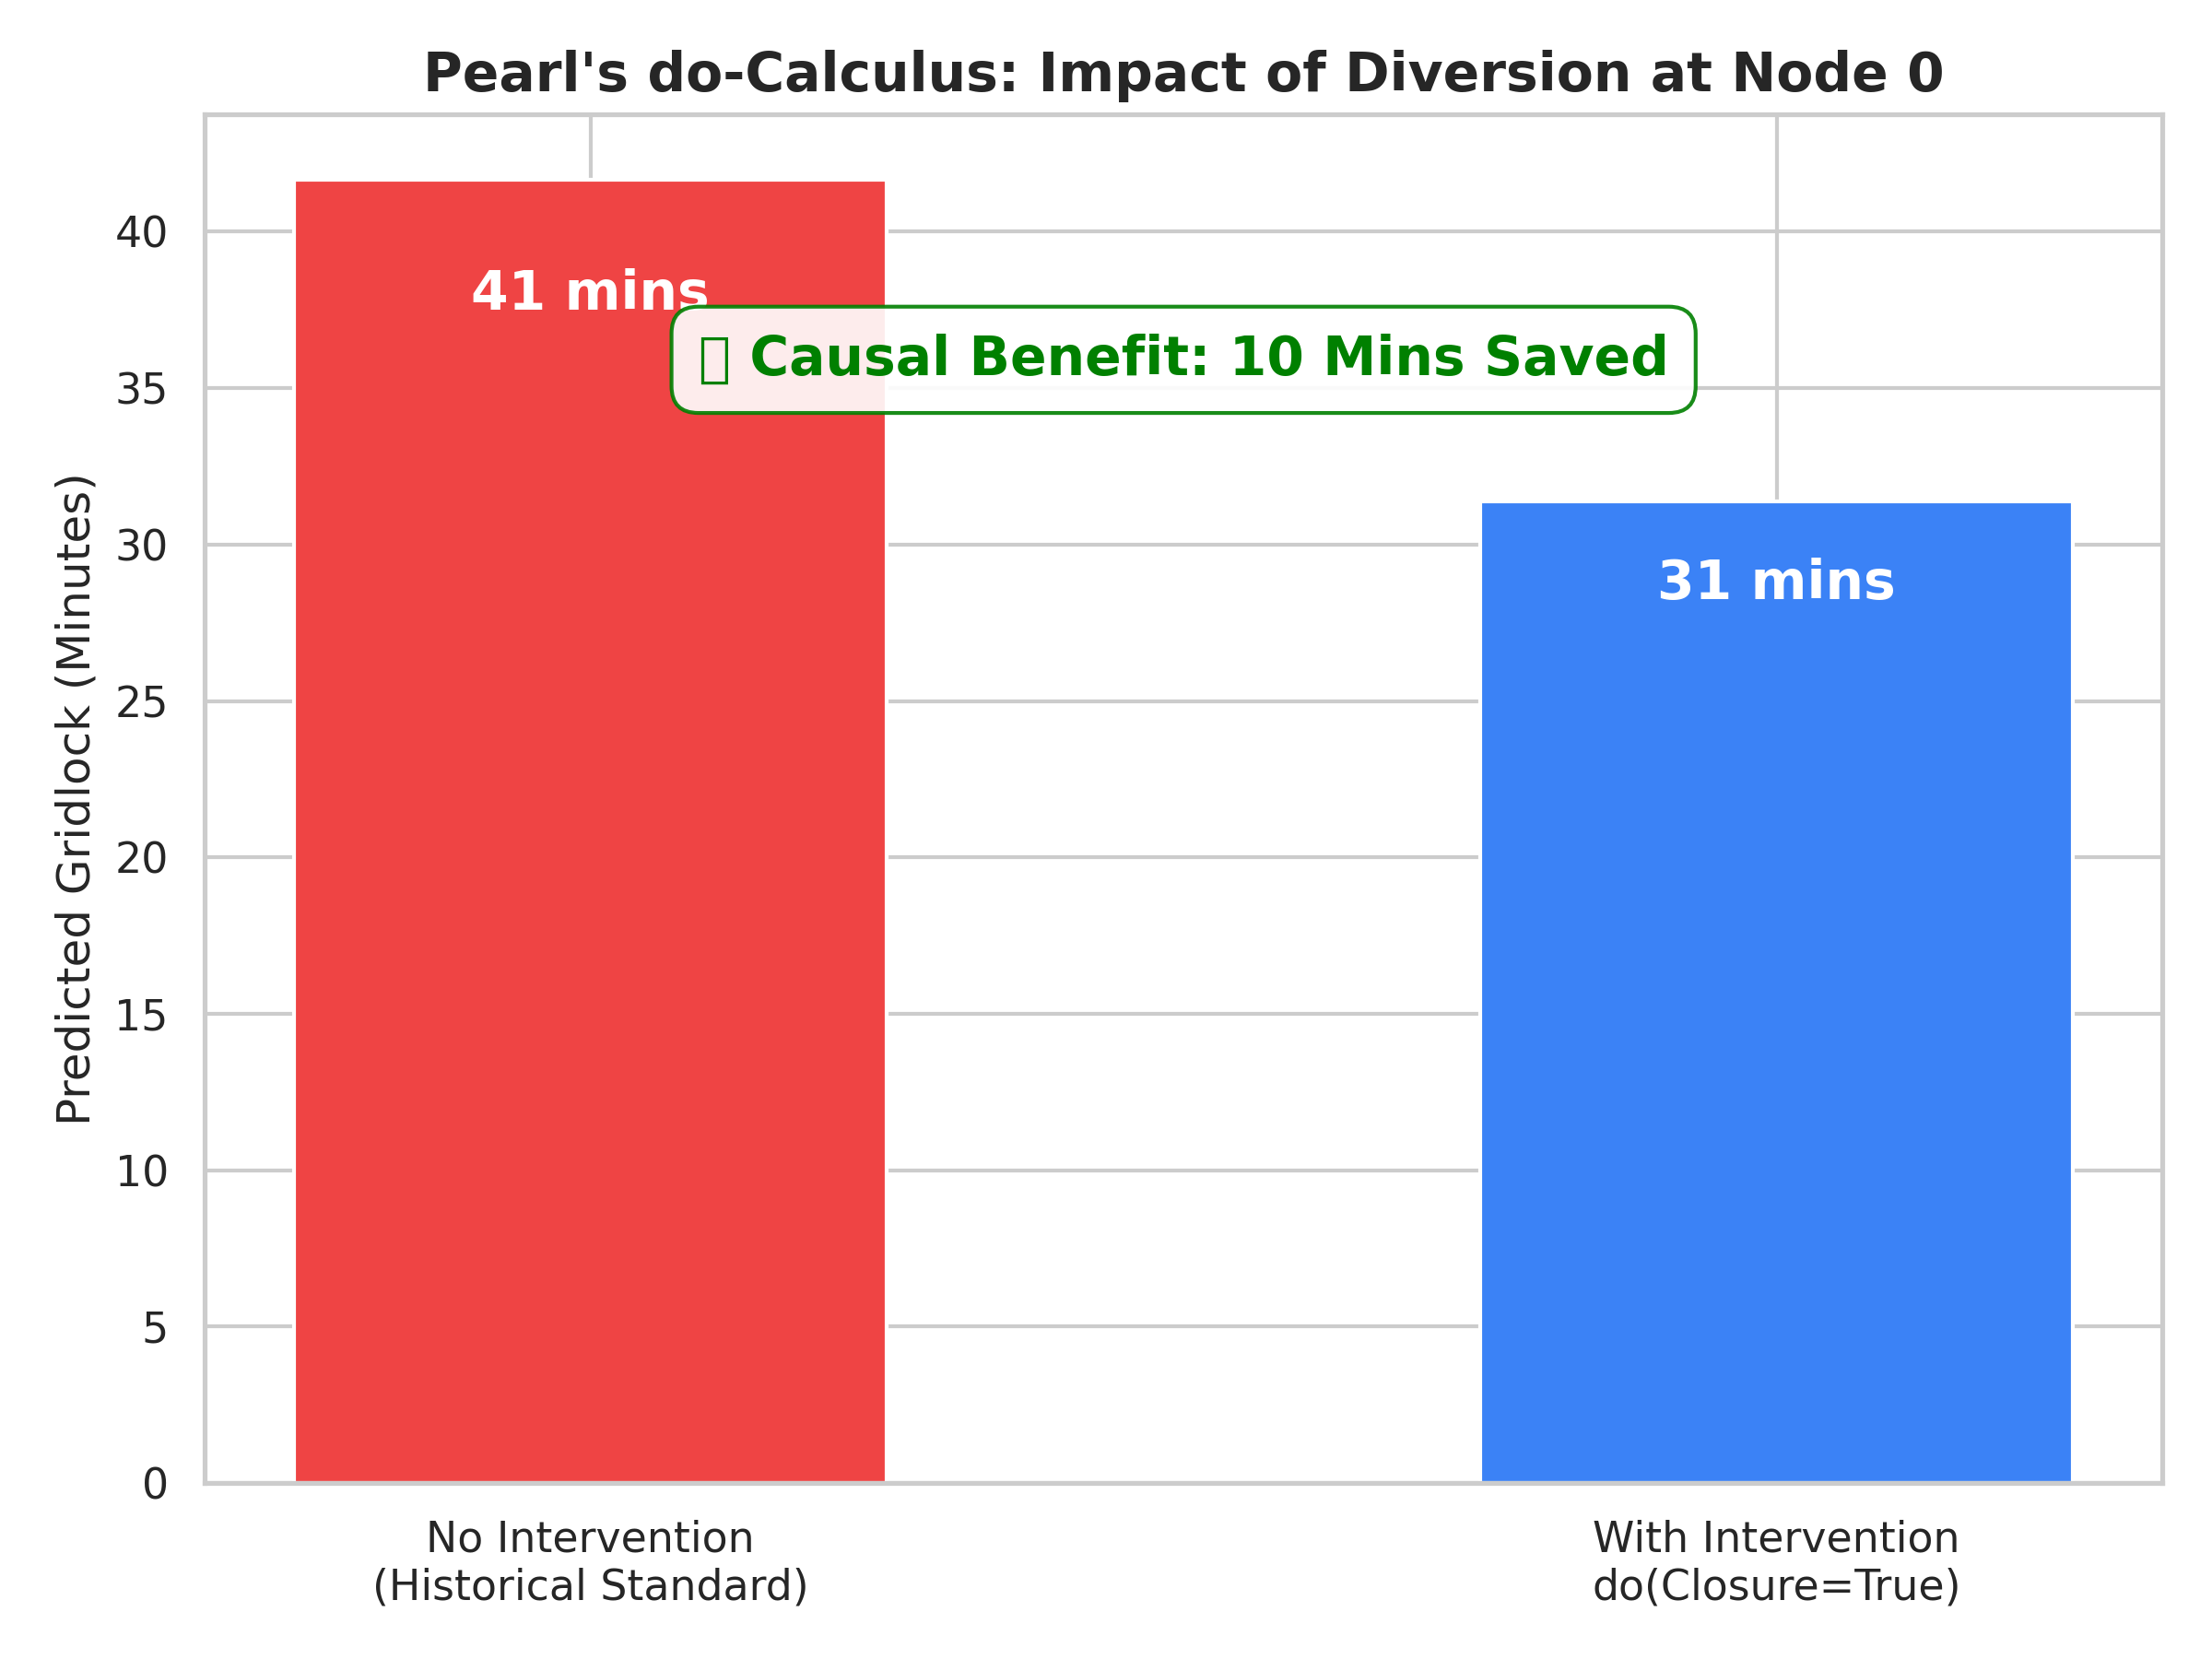
\includegraphics[width=\textwidth]{ml_notebook/08_Causal_Intervention_Impact.png}
            \vspace{0.2em} \\ \scriptsize Simulation projecting significant reduction in gridlock.
        \end{column}
        \begin{column}{0.5\textwidth}
            \centering
            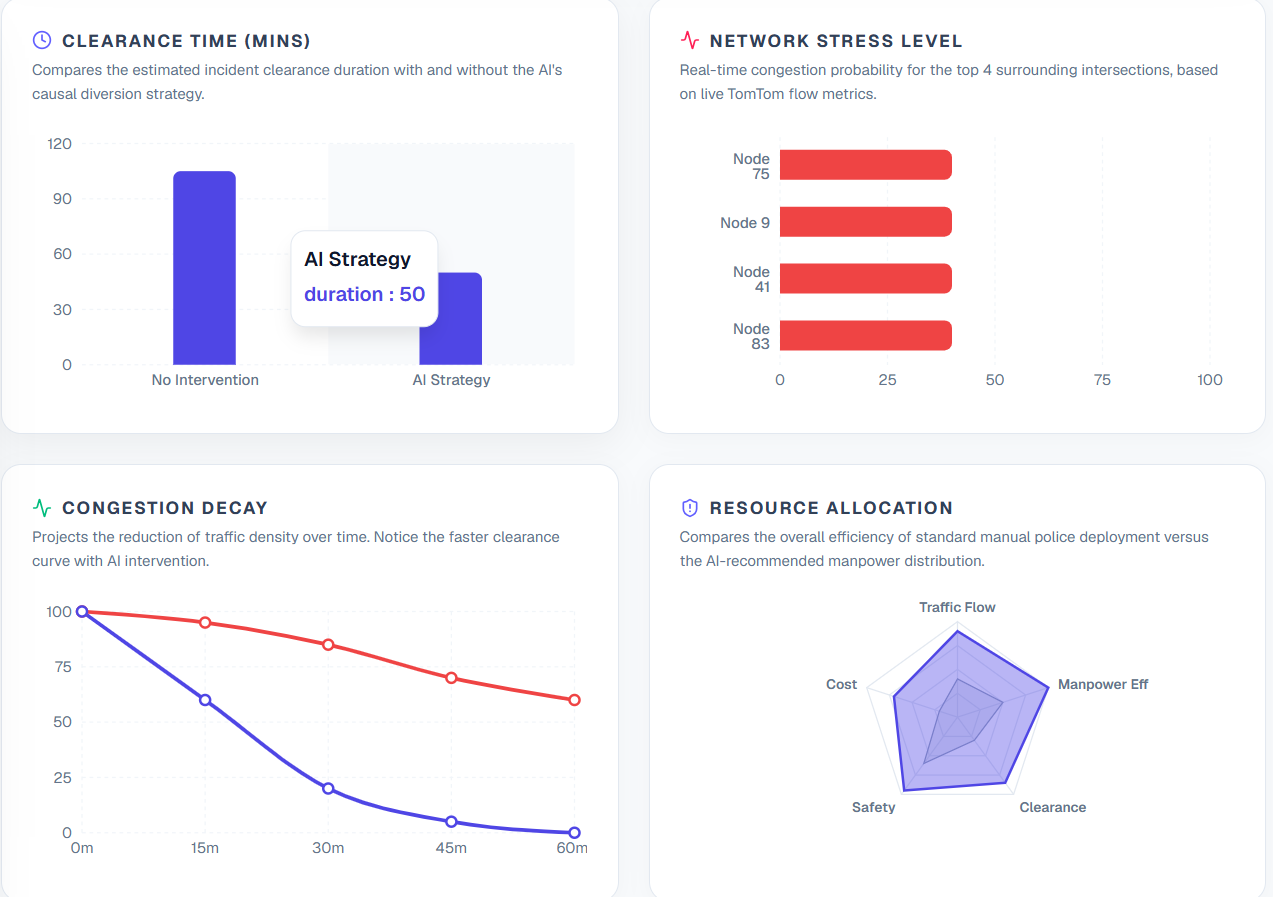
\includegraphics[width=\textwidth]{ui_shots/metrics_ui.png}
            \vspace{0.2em} \\ \scriptsize Return on Intervention (ROI) evaluated in real-time.
        \end{column}
    \end{columns}
\end{frame}

% Slide 9: Tech Stack & Future Scope
\begin{frame}{Tech Stack \& Future Scope}
    \textbf{Modern Technology Stack}
    \begin{itemize}
        \item \textbf{Machine Learning:} PyTorch, Hugging Face Transformers (BERT)
        \item \textbf{Backend \& Inference:} FastAPI, Groq Cloud (LLaMA-3 8B)
        \item \textbf{Mapping \& Routing:} MapmyIndia APIs (Mappls)
        \item \textbf{Frontend Application:} Next.js, React, Recharts, Leaflet
    \end{itemize}
    
    \vspace{1em}
    \textbf{Future Scope \& Scalability}
    \begin{itemize}
        \item \textbf{Physical Infrastructure Integration:} Interfacing with adaptive traffic light grids to autonomously execute pre-emptive signal alterations.
        \item \textbf{Live CCTV Vision Processing:} Ingesting real-time video streams via edge-AI to dynamically update the causal graph based on ground-truth density.
        \item \textbf{Predictive Weather Context:} Incorporating localized meteorological data APIs to adjust congestion decay rates dynamically during storms.
        \item \textbf{Cross-Agency Communication:} Automated alert dissemination bridging police dispatch systems, fire departments, and ambulance fleets.
        \item \textbf{V2X (Vehicle-to-Everything) Communication:} Pushing micro-diversion routes directly to connected vehicles' navigation systems dynamically.
        \item \textbf{Public Sentiment Analysis Integration:} Scanning social media streams in real-time to adjust crowd sentiment multipliers affecting the severity index.
    \end{itemize}
\end{frame}

\end{document}
